% \documentclass{beamer}
% \usepackage{multicol}
% \usepackage{graphicx}
% \graphicspath{{./fig/}}
% \usetheme{material}


% \begin{document}

\section{3D-PTV Overview}

\begin{frame}[label=ptv-1]{Fluid dynamicists in the audience?}
\centering\cardImg[height]{7j34up.jpg}{.8\textwidth}
\end{frame}


\begin{frame}[label=ptv-21]{3D-PTV overview}
\begin{multicols}{2}
\begin{card}[What is 3D-PTV]
3D-PTV is a technique that allows tracking of particles in three-dimensional space for improved fluid dynamics understanding, using the Lagrangian framework
\end{card}
\begin{card}[How does it work?]
Multiple 2D projections of the particles are obtained and overlapped to create 3D reconstruction. Software than tracks the particles' positions through sequential images over time. 
\end{card}
\end{multicols}
\end{frame}


%
\begin{frame}[label=ptv-211]{Overview from Shr\"{o}der and Schanz, Annu. Rev. Fluid Mech. 2023}
\cardImg{shroder.jpeg}{\textwidth}
\end{frame}

\begin{frame}[label=ptv-3]{What is this Lagrangian framework?}
\centering\cardImg{art}{0.8\textwidth}
\vspace{-.3cm}
\begin{cardTiny}
``Marianthe'' invited people inside turbulent forms to experience them as
if they were a particle borne along in the flow. Athena
Tacha (1985), \href{http://nautil.us/issue/15/turbulence/the-scientific-problem-that-must-be-experienced}{``Nautilus'' by Philip Ball}
\end{cardTiny}
\end{frame}
%

\begin{frame}[label=ptv-4]{Quick intro to 3D-PTV}
\cardImg{ptv-scheme}{1.0\textwidth}
\end{frame}
% % 
% % %
% \begin{frame}[label=ptv-2]{Basic steps}
% \begin{columns}[t]
% 	\begin{column}{0.4\textwidth}
% 		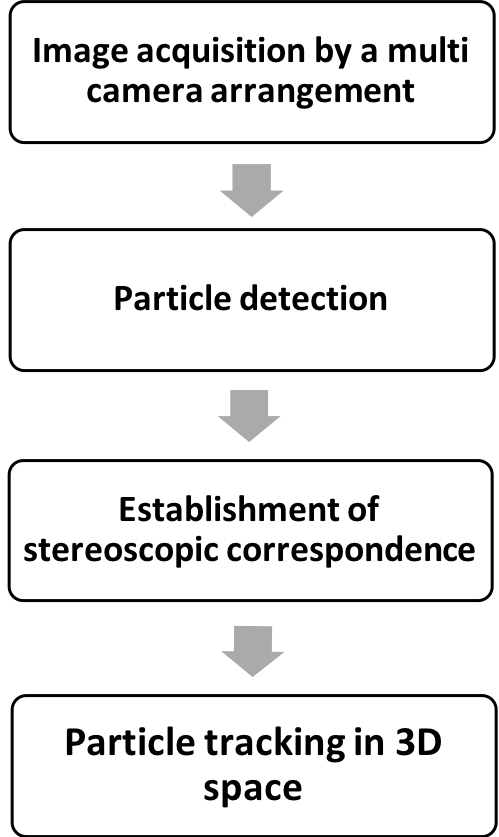
\includegraphics[height=.8\textheight]{ptv_blocks}
% 	\end{column}
% 	\begin{column}{0.3\textwidth}
% 		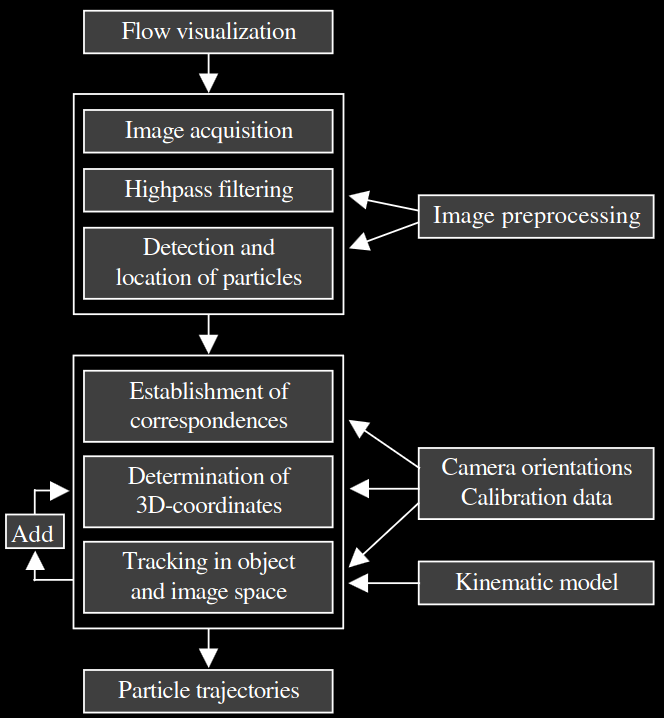
\includegraphics[height=.8\textheight]{ptv_steps}
% 	\end{column}
% \end{columns}
% \end{frame}


\begin{frame}[label=ptv-2]{Basic steps of 3D-PTV}
\centering\cardImg[height=.8\textheight]{ptv_steps}{\textwidth}
\end{frame}

% %%
% \begin{frame}[label=ptv-22]{Basic steps}
% \begin{multicols*}{2}
% 		\cardImg[height]{ptv_blocks}{.49\textwidth}
% 		\cardImg[height]{ptv_steps}{.49\textwidth}
% \end{multicols*}
% \end{frame}

\begin{frame}[label=ptv-5]{Epipolar geometry}
\centering\cardImg{epipolar1}{1\textwidth}
\end{frame}

\begin{frame}[label=ptv-51]{Multi-view epipolar geometry}
\centering\cardImg{epipolar}{\textwidth}
\end{frame}

\begin{frame}[label=ptv-51]{Multi-view epipolar geometry}
\centering\cardImg{stereo_matching}{\textwidth}
\end{frame}

\begin{frame}[label=ptv-55]{Multi-view epipolar geometry depends on calibration}
\centering\cardImg{calibration1}{\textwidth}
\end{frame}

	

\begin{frame}[label=ptv-6]{Four frames sliding tracking}
\centering\cardImg{tracking}{1\textwidth}
\end{frame}

\begin{frame}[label=ptv-61]{Tracking in 2D space}
\centering\cardImg[height=.8\textheight]{tracking_in_image_space_projection}{1\textwidth}
\end{frame}


\begin{frame}[label=ptv-61]{Tracking in 2D space}
	\centering\cardImg[height=.8\textheight]{tracking_in_image_space}{1\textwidth}
\end{frame}

\begin{frame}[label=ptv-61]{Tracking in 3D }
	\centering\cardImg[height=.8\textheight]{tracking_in_3d_space}{1\textwidth}
\end{frame}

\begin{frame}[label=ptv-61]{Tracking in both 2D and 3D}
	\centering\cardImg[height=.8\textheight]{image_space_tracking}{1\textwidth}
\end{frame}

			

\begin{frame}[label=ptv-7]{The results are Lagrangian trajectories}
\centering
\cardImg{lagrangian_trajectory}{.49\textwidth}
\cardImg{particle_trajectories}{.49\textwidth}
\end{frame}

\begin{frame}[label=ptv-71]{Two frame PTV is Eulerian, not Lagrangian}
\centering\cardImg{eulerian_vs_lagrangian}{\textwidth}
\end{frame}

\begin{frame}[label=ptv-8]
\frametitle{Time-resolved is tautology, real-time is real :) }
\begin{enumerate}
\item Time resolved PTV is tautology - to track objects we have to resolve its position in time :) 
\item Real time is not at the velocity of the particle, but during the experiment: we get trajectories on the screen when the flow is moving (not the same flow)
\end{enumerate}
\end{frame}

 % \end{document}